\chapter{Validation of TRACS for irradiated silicon detectors}
\label{sec:TRACSvalidity}

A first way to attest the validity of TRACS results after the implementation of radiation damage is to compare them to other measurements already published and accepted. In \cite{Pholsen} it is shown how a linear parametrisation of the \neff can be used to reproduce measurements of irradiated sensors accurately.

These results will be used as the first test to check TRACS simulations. It is also necessary to conduct a controlled test in which TRACS is compared against data measured in the laboratory. By doing this the author can attest the validity of the measuring and simulation procedures. This task will be the second and last test to validate TRACS results.

TRACS is able to reproduce any kind of TCT measurement provided the carrier distribution inside the detector. The choice was made to perform red-TCT measurements in the TCT+ setup at CERN-SSD\cite{ssd}. In particular bottom-TCT was chosen after several measurements since it showed clear signs of radiation damage in the form of the DP explained in section \ref{sec:signalDeg}. 

It is important to note that TRACS needs to be given between 3 and 7 different parameters to perform a correct simulation of an irradiated silicon detector. This complexity calls for automated fitting software that is planned to be developed but is not available at the time of writting this project.

It is for this reason that comparison with measurements will only be performed with one detector and using only one technique. Parameters will be optimised manually by trial-and-error. The results of such manual fit are not expected to be quantitatively accurate but only to reproduce qualitatively the measuremetns. The simulation-measurement comparison will only attest TRACS validity but not TRACS accuracy.

The detector used was a diode previously irradiated to $10^{15} neq$. It has a  1cmx1cm surface with 300 $\mu$m width with a structure similar to that explained in section \ref{REFERENCIA A DEFINIR}. The diode was also subject to the standard annealing process after irradiation and stored in a fridge to ensure constant low temperatures and prevent radiation effects to evolve over time. 


\section{Experimental procedure} % (fold)
\label{sec:ExpProc}

For the comparison between TRACS and published simulations the only steps needed to be taken were digitalising the publised simulations and performing the simulations using TRACS with the same parameters as in the reference. 

The setup used for the red-TCT measurements was the one described in section \ref{sec:TCTsetup}. Using the bottom-TCT configuration a voltage scan was performed recording the transients generated with bias voltage ranging from 0V to 140V in steps of 10V. The measurements were performed with the detector at fixed temperature T = 273K. 

% MOAR DATA?

% section Experimental setup (end)
\section{Results and comparison} % (fold)
\label{sec:comparison}

Comparison will be presented in two different manners. First a comparison of each set of data (measurements and simulations) will be presented in separated plots. This will illustrate similarities in the trends followed by the transients when \vias is increased. A few sample transients will be selected for direct comparison between measurements and simulations. 

Simulation and measurements will be plotted together with different plots for each of the selected voltages. This will allow to compare the specific features of the transients and establish the agreement between simulations and measurements. The data has been normalised to the maximum value of the histograms. In this way the direct comparison is easier and the intensities of the laser are factores out of it.  

\subsection{Comparison between TRACS and already existing simulations}

To compare TRACS to other simulations data from \cite{Pholsen} will be used. In this doctoral thesis, the \neff is parametrised as a linear function of depth. Since the raw data is not published, it was needed to digitalise the plots published in the reference. For said task an online tool was used \cite{digitiser}

Transients from \cite{Pholsen} also include measured data that supports the validity of the simulation presented there. To reproduce the measurements we used a linear parametrisarion.

\begin{figure}[H]
	\centering
	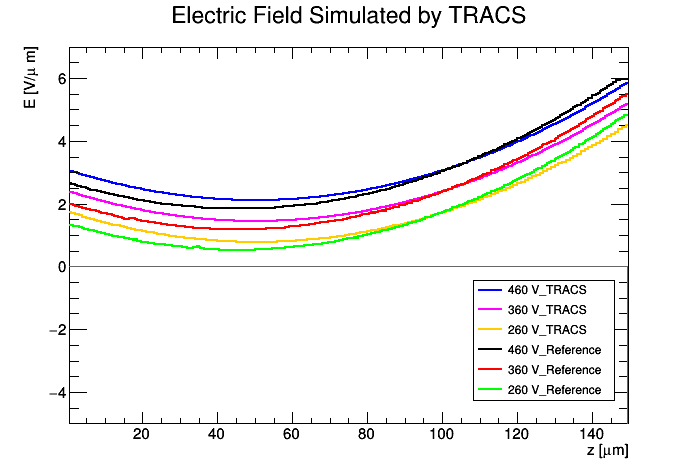
\includegraphics[width=0.8\textwidth]{Pohlsen_fields.png}
	\label{fig:CompFields}
	\caption{Electric field inside the diode as a function of depth. Simulations from \cite{Pohlsen} and TRACS are plotted together for comparison. Agreement between both simulations is good as expected.}
\end{figure}

The transients presented in the reference were also simulated with TRACS and compared. The reader should note that the trapping simulation is different between both simulators with TRACS having a constant $\tau$ whilst the reference uses a field-dependant $\tau$. Results are therefore expected to not be the same but compatible.

\begin{figure}[H]
	\centering
	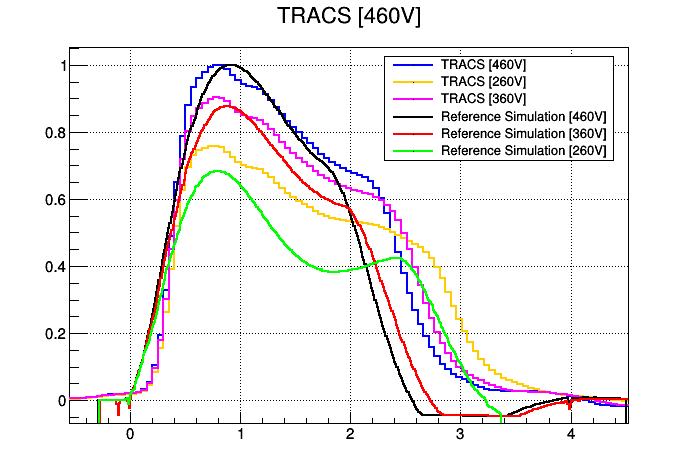
\includegraphics[width=0.8\textwidth]{Pohlsen_scr.png}
	\label{fig:mues2}
	\caption{Transient currents generated by top-TCT measurements (continuos line) and simulations(histogram). TRACS uses a different trapping parametrisation yielding slightly different results while maintaining the general features of the measurements from \cite{Pohlsen}}
\end{figure}


\subsection{Comparison between simulations and laboratory measurements}

%Deberia haber comentado en la parte de TRACS sobre que TRACS no simula difusion?

In order to reproduce the transients obtained in the laboratory the trial-and-error method was performed manually. The results presented in this section are considered to be a good representation of the measured detector but not a perfect match. The chosen \neff parametrisation was the Trilinear form. A table with the 8 defining values for the chosen \neff are presented below together with a plot of the \neff distribution as a function of depth. Trapping constant was chosen to be: $\tau = 5 ns$

\begin{centering}
\begin{tabular}{c}
	
	% TABLA

\end{tabular}
\end{centering}

The data measure by the author is presented now. In the following plot all the transients measured in the laboratory can be seen together. It can be seen that the Double Peak feature appears only for $\vias \geq 80 V$. This value of $\vias$ can be considered a good estimation of the $V_{dep}$. It can be seen that transients get shorter in time with increasing voltages with the second peak getting higher with higher voltages. 

\begin{figure}[H]
	\centering
	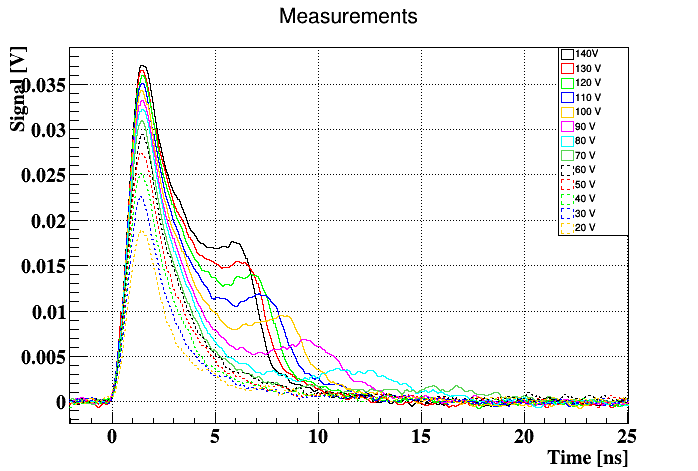
\includegraphics[width=0.9\textwidth]{c1.png}
	\label{fig:mues2}
	\caption{Measurements performed in the SSD facilities are presented here. The irradiated diode presents signs of radiation damage (DP). This transients serve as reference to compare with TRACS simulations}
\end{figure}
				
TRACS simulations are presented now in a similar manner as the measurements. Comparison of the transient response to higher voltages can be done with these plots. It can be seen that TRACS simulations follow a similar trend of shorter transients and higher second peaks with increasing voltages.

\begin{figure}[H]
	\centering
	\centering
	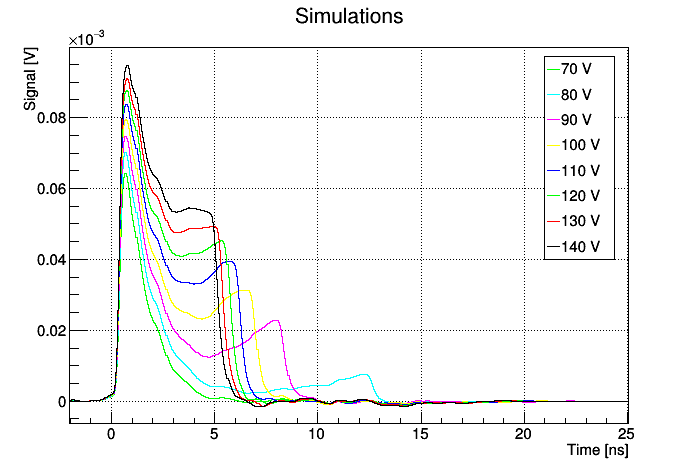
\includegraphics[width=0.9\textwidth]{AllSims.png}
	\label{fig:mues2}
	\caption{Simulations performed by TRACS are presented here. The triple linear approximation was used for the simulation. The simulated transients present similar features as the measured data.}
\end{figure}

No transients below $80V \approx V_{dep}$ were simulated because TRACS does not simulate diffusion inside the detector. Together with the fact that illumination is done in the non depleted area for $V < 80V$ this means that any simulation done in TRACS for voltages under $V_{dep}$ will have no physical meaning.

These two plots allow to see how TRACS reproduces the trends of the transients with different voltages but direct comparison of the transients can be difficult. In the following plots a direct comparison of selected transients will be presented for a more comprehensive look at the transient features and how TRACS is able to simulate measurements.

From the previous voltage scans, three transients have been selected. The three voltages selected are 80V, 100V and 140V. 

\begin{figure}[H]
	\centering
	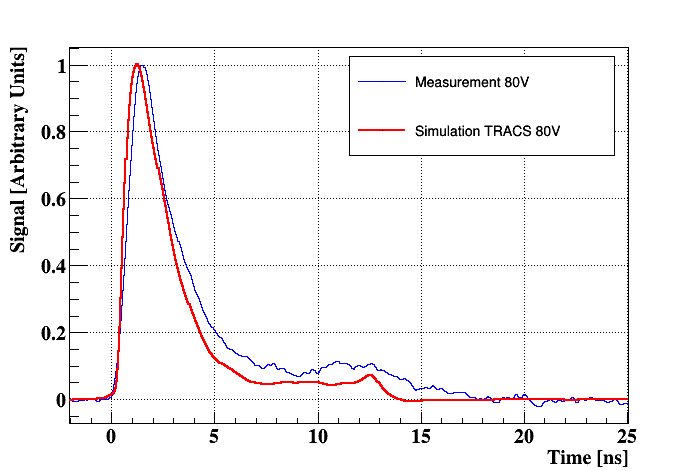
\includegraphics[width=0.9\textwidth]{80V.png}
	\label{fig:mues2}
	\caption{Comparison of the measured transients (blue line) and the simulations from TRACS (red line) for a bias voltage $V = 80V$. Both transients present similar features and can be considered compatible.}
\end{figure}


\begin{figure}[H]
	\centering
	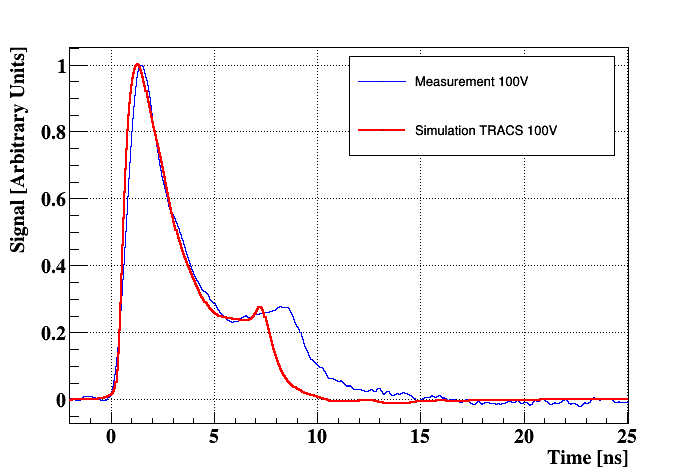
\includegraphics[width=0.9\textwidth]{100V.png}
	\label{fig:mues2}
	\caption{Comparison of the measured transients (blue line) and the simulations from TRACS (red line) for a bias voltage $V = 100V$. Both transients present similar features and can be considered compatible.}
\end{figure}

% Is it OK to copy the captions?

\begin{figure}[H]
	\centering
	\includegraphics[width=0.9\textwidth]{140V.png}
	\label{fig:mues2}
	\caption{Comparison of the measured transients (blue line) and the simulations from TRACS (red line) for a bias voltage $V = 140V$. Both transients present similar features and can be considered compatible.}
\end{figure}

Looking at the three comparison figures it is easy to see that TRACS simulations show similar features and behaviour as the measurements. The fact that the simulations don't match perfectly the measurements can be attributed to the shapping algorithm (the transfer function of the amplifier used in the measurements was not available for the simulations) and also to the only approximate fitting of the parameters, as we have discussed before. Better agreement between simulations and measurements can be expected if this problems are addressed.
% section future_projection (end)

